\documentclass[graybox]{styles/svmult}

\usepackage{mathptmx}
\usepackage{helvet}
\usepackage{courier}
\usepackage{type1cm}

\usepackage{makeidx}
\usepackage{graphicx}
\usepackage{placeins}

\usepackage{multicol}
\usepackage[bottom]{footmisc}

\usepackage{listings}

\makeindex

\begin{document}

\title*{Genetic Algorithm Selection Operator \\ Based on Recursion and Brute-Force}
\titlerunning{GA Selection with Recursion \& Brute-Force}

\author{Petar Tomov, Iliyan Zankinski, Todor Balabanov}
\authorrunning{P. Tomov et al.} 

\institute{Petar Tomov \at Institute of Information and Communication Technologies - Bulgarian Academy of Sciences \\ acad. Georgi Bonchev Str., block 2, 1113 Sofia, Bulgaria \email{p.tomov@iit.bas.bg}
\and Iliyan Zankinski \at Institute of Information and Communication Technologies - Bulgarian Academy of Sciences \\ acad. Georgi Bonchev Str., block 2, 1113 Sofia, Bulgaria \email{iliyan@hsi.iccs.bas.bg}
\and Todor Balabanov \textsuperscript{0000-0003-3139-069X} \at Institute of Information and Communication Technologies - Bulgarian Academy of Sciences \\ acad. Georgi Bonchev Str., block 2, 1113 Sofia, Bulgaria \email{todorb@iinf.bas.bg}}
%
% Institute of Information and Communication Technologies
% Bulgarian Academy of Sciences
% acad. Georgi Bonchev Str., block 2, office 514, 1113 Sofia, Bulgaria
% iict@bas.bg
% http://www.iict.bas.bg/
%

\maketitle

\abstract*{In the area of global optimization genetic algorithms are meta-heuristics provoked by the processes in the biological evolution. Calculations are separated in three basic operations - crossover, mutation and selection. The first and second add new individuals to the population and selection is expected to keep better parents in the population. For the last five decades different selection operators are introduced in the literature. The most popular are: Proportional Selection, Tournament Selection, Rank-Based Selection, Boltzmann Selection, Soft Brood Selection, Disruptive Selection, Nonlinear Ranking Selection and Competitive Selection. In this study a new selection operator based on recursive generations creation is proposed. In every level of recursive descent all local individuals are recombined with each other (brute-force) and only the best found individual is sent to the population of the higher level.}

\abstract{In the area of global optimization genetic algorithms are meta-heuristics provoked by the processes in the biological evolution. Calculations are separated in three basic operations - crossover, mutation and selection. The first and second add new individuals to the population and selection is expected to keep better parents in the population. For the last five decades different selection operators are introduced in the literature. The most popular are: Proportional Selection, Tournament Selection, Rank-Based Selection, Boltzmann Selection, Soft Brood Selection, Disruptive Selection, Nonlinear Ranking Selection and Competitive Selection. In this study a new selection operator based on recursive generations creation is proposed. In every level of recursive descent all local individuals are recombined with each other (brute-force) and only the best found individual is sent to the population of the higher level.}

\section{Introduction}
\label{sec:1}

Genetic algorithms\index{genetic algorithms} are a heuristic tool for global optimization \cite{balabanov-01}. Because many randomly generated numbers are applied to them, genetic algorithms have a stochastic nature and do not guarantee a global optimum achievement. Also, at each run the results may differ \cite{balabanov-02}, but there are great opportunities for effective implementation in the form of parallel calculations \cite{balabanov-03}. The ideas behind genetic algorithms are inspired by the theory of natural evolution. A single point in a multidimensional space (solution space) is described as a vector. One vector represents one individual in the population of the genetic algorithm \cite{balabanov-04}. There is no universal theory for determining population size, but most often it is up to 100 individuals \cite{alander-01}. Each individual in the population is a subject of evaluation, which is obtained by calculating the target function. The vector of the decision space is fed to the input of the target function and after its calculation a single value is produced. Different tasks may require searching of a minimum or a maximum value. The closer the calculated value of the individual is to the desired optimum, the better its fitness is. More viable individuals are more often chosen to create a generation. The offspring undergoes two common operations - crossover and mutation. Crossing helps to search the solution space extensively while the mutation helps with finer examination of the surroundings of already crossed individuals. Genetic algorithms are subject to research from the middle of the last century, but there are still areas in which their productivity can be improved. The present study focuses on the selection operation and how this operation can improve the search for a global optimum when functions with a large number of local optima are investigated.

Parent selection for offspring production can be done in many different strategies \cite{balabanov-05}, which have been extensively explored in the literature. The most important responsibility in mating is to use better individuals from the population more often in the hope that they will lead to even better solutions. If parents are chosen at random (Random Search), reaching sub-optimal, but acceptable solutions would be too slow \cite{wang-01}. One of the earliest proposals for selection is Proportional Selection \cite{back-01}. In this strategy, each individual in the population receives a probability of crossover proportional to the fitness value they have achieved. Another popular strategy is Tournament Selection \cite{miller-01}, in which a subset of randomly selected individuals only one is nominated on a competitive basis (the best candidate among them). Rank-based Selection is a third popular strategy \cite{grefenstette-01}. In it each individual is determined by their likelihood of participating in future offspring by the rank (indirect fitness) that is present in the population. Simulated annealing is at the heart of Boltzmann Selection \cite{goldberg-01}. In this type of selection, the winner is determined after a series of Boltzmann experiments.

There are many varieties or modifications to the above mentioned selection strategies. This study examines a recursive descent-based selection operation \cite{gelfand-01} by a hierarchy of generations among which, with total exhaustion, \cite{fellows-01} only one individual participates in the higher level of recursion.

The article is organized as follows: Introduction defining the scope of the study; Proposal for the operation selection with recursion and complete exhaustion; Experiments and results illustrating the proposed operation; Conclusion, with a summary of the research done and suggestions for future development.

\section{Brute-Force and Recursion based Selection Operator}
\label{sec:2}

This scientific study proposes a selection operation used in genetic algorithms just before recombination operations are performed. In the presence of a population of size n, there are numerous ways to select parent individuals to be used for a new generation creation. In most implementations of genetic algorithms, selection is performed on the basis of some calculated probability \cite{matsui-01}. In this study, an approach was chosen at the other extreme (Listing \ref{fig:1}), namely that each individual of a particular generation recombines with each other (including himself).

\begin{figure}[b]
\sidecaption
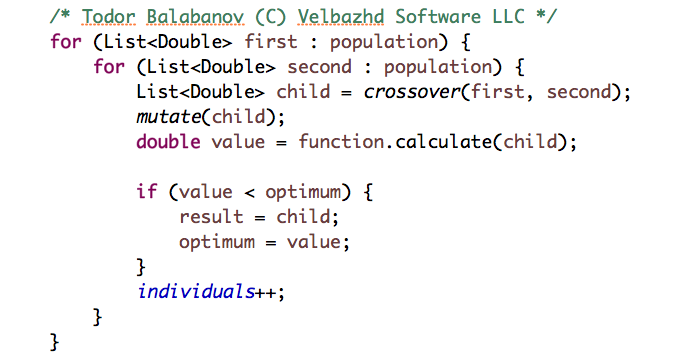
\includegraphics[width=1.0\textwidth]{images/fig09}
\caption{Brute-force based recombination}
\label{fig:1}
\end{figure}
%\FloatBarrier

This selection operation is completely exhausted and all individuals participate equally, with equal chances for offspring. Of all the newly generated offspring, only one (the best) individual is sent one level up (Listing \ref{fig:2}) into the hierarchy of recursive calls.

\begin{figure}[b]
\sidecaption
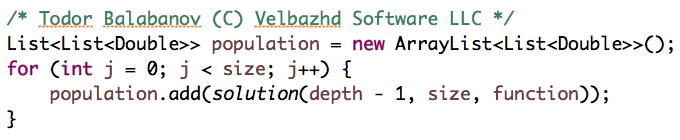
\includegraphics[width=1.0\textwidth]{images/fig10}
\caption{Promotion of best found individual in a particular recursive level}
\label{fig:2}
\end{figure}
%\FloatBarrier

For each level of the hierarchy, a population is created with individuals sent from the lower level. In this way, each population is formed by a plurality of lower-level individuals. The population at the bottom of the recursion is filled with randomly generated individuals (Listing \ref{fig:3}).

\begin{figure}[b]
\sidecaption
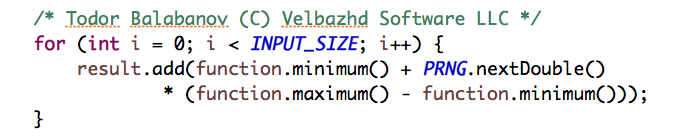
\includegraphics[width=1.0\textwidth]{images/fig11}
\caption{Random individuals are created at the bottom of the recursion}
\label{fig:3}
\end{figure}
%\FloatBarrier

Individuals generated at the bottom of the recursion are not evaluated through fitness function, because it does not matter what the value would be.

\section{Experiments and Results}
\label{sec:3}

The experiments were performed with a desktop computer system having the following parameters: Intel Core i5, 2.3 GHz, 2 Cores, 8GB RAM and Mac OS X 10.13.6, Oracle Java 1.8.0-91 \cite{balabanov-06}. For the experiments performed, two functions with multiple local and global optima were selected - Rastrigin (Fig. \ref{fig:4}) and Griewank (Fig. \ref{fig:5}), which make it difficult to find the global minimum due to the presence of multiple local ones \cite{balabanov-07}.

\begin{figure}[b]
\sidecaption
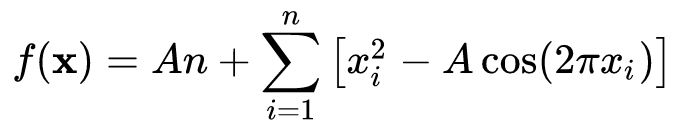
\includegraphics[width=1.0\textwidth]{images/fig01a}
\caption{Rastrigin function equation}
\label{fig:4}
\end{figure}
%\FloatBarrier

Both selected features have a distinct global minimum. Multiple local lows are available for both functions. Fig. \ref{fig:3} and \ref{fig:4} show graphs of functions in two-dimensional space. For the experiments performed, the functions are used in a one hundred-dimensional space. The availability of one hundred free variables makes it possible to maximize the use of genetic algorithms to find optimal solutions in multidimensional spaces.

\begin{figure}[b]
\sidecaption
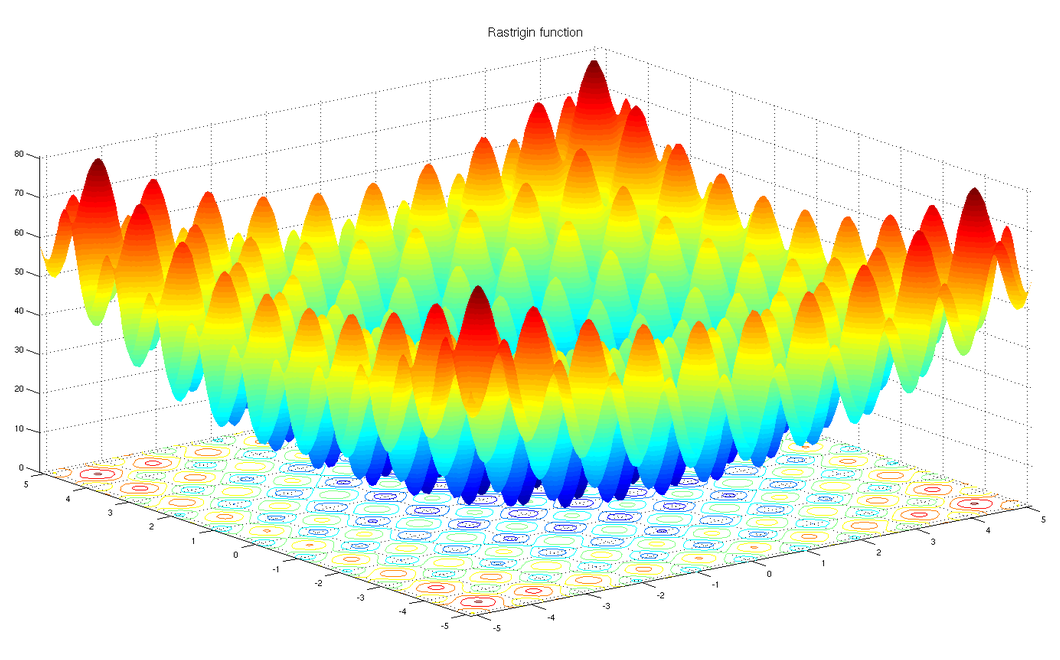
\includegraphics[width=1.0\textwidth]{images/fig01b}
\caption{Rastrigin function in 2D case}
\label{fig:5}
\end{figure}
%\FloatBarrier

In both functions, the presence of a parabolic component defines the shape of the valley, and the cosine gives the shape of local elevations.

\begin{figure}[b]
\sidecaption
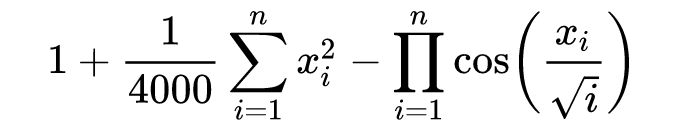
\includegraphics[width=1.0\textwidth]{images/fig02a}
\caption{Griewank function equation}
\label{fig:6}
\end{figure}
%\FloatBarrier

The experiments take into account the execution time of the optimization algorithm, the number of estimated individuals in the population, as well as the closest to the optimal solution calculated value.

\begin{figure}[b]
\sidecaption
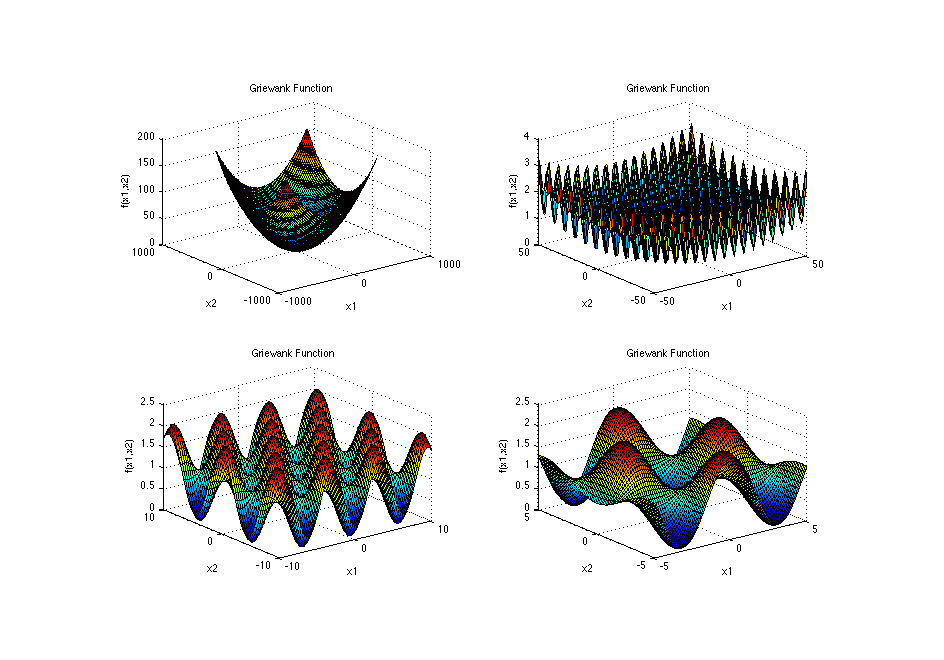
\includegraphics[width=1.0\textwidth]{images/fig02b}
\caption{Griewank function in 2D case}
\label{fig:7}
\end{figure}
%\FloatBarrier

All experiments were performed under different configurations for depth of recursion and population size at each hierarchical level in recursive calls. Values from 2 to 8 were examined as the depth of recursion and values from 2 to 11 were studied as population size (Tables \ref{fig:8} and \ref{fig:9}).

\begin{figure}[b]
\sidecaption
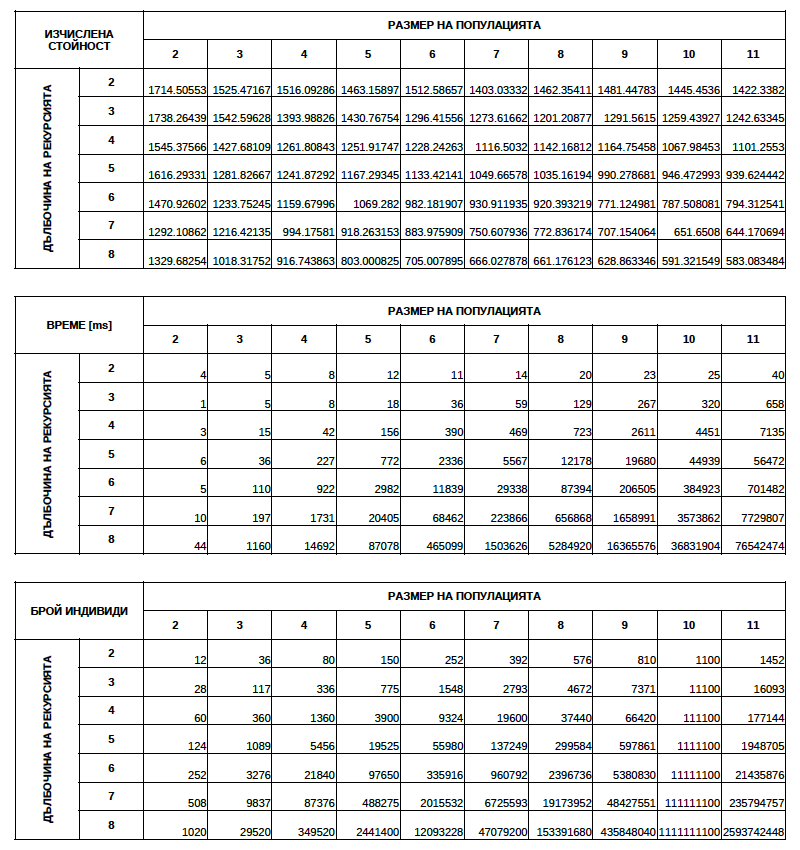
\includegraphics[width=1.0\textwidth,height=0.45\textheight]{images/fig12}
\caption{Rastrigin measured results}
\label{fig:8}
\end{figure}
%\FloatBarrier

\begin{figure}[b]
\sidecaption
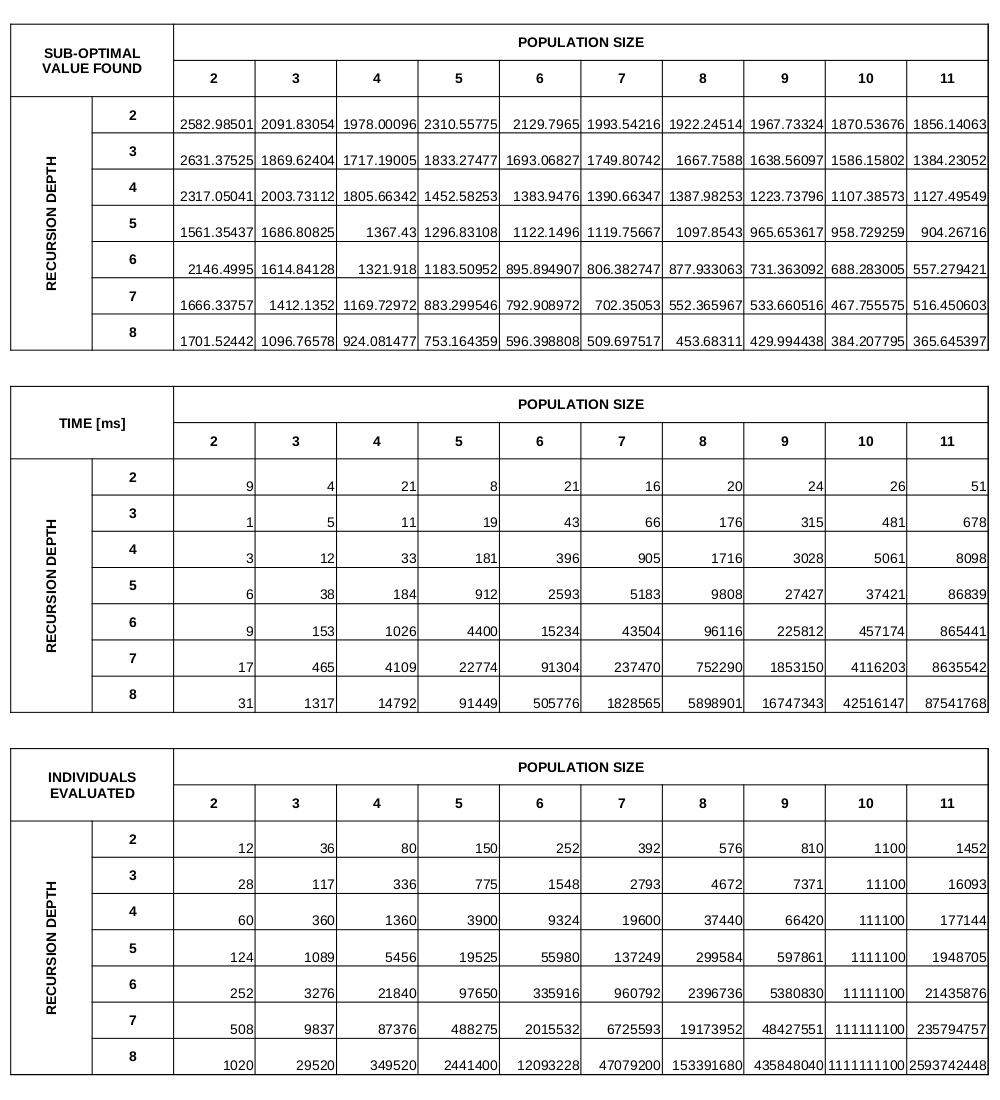
\includegraphics[width=1.0\textwidth,height=0.45\textheight]{images/fig13}
\caption{Griewank measured results}
\label{fig:9}
\end{figure}
%\FloatBarrier

From the results presented, it is clear that with increasing population size and recursion depth, the proposed selection operation leads to solutions that are closer to the global optimum. Because at each hierarchical level each individual intersects with each other, this leads to too much time consumption and asymptotic complexity of $O(n^2)$, for n individuals in one generation.

\begin{figure}[b]
\sidecaption
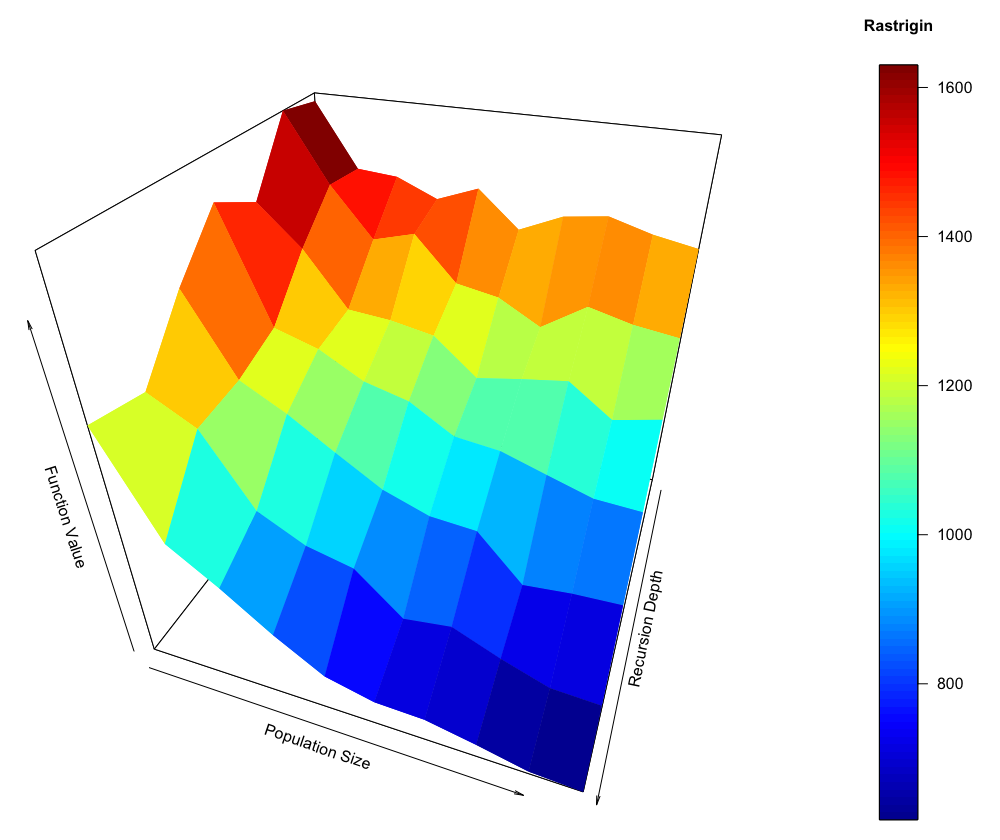
\includegraphics[width=1.0\textwidth,height=0.45\textheight]{images/fig03}
\caption{Rastrigin sub-optimal solutions found}
\label{fig:10}
\end{figure}
%\FloatBarrier

\begin{figure}[b]
\sidecaption
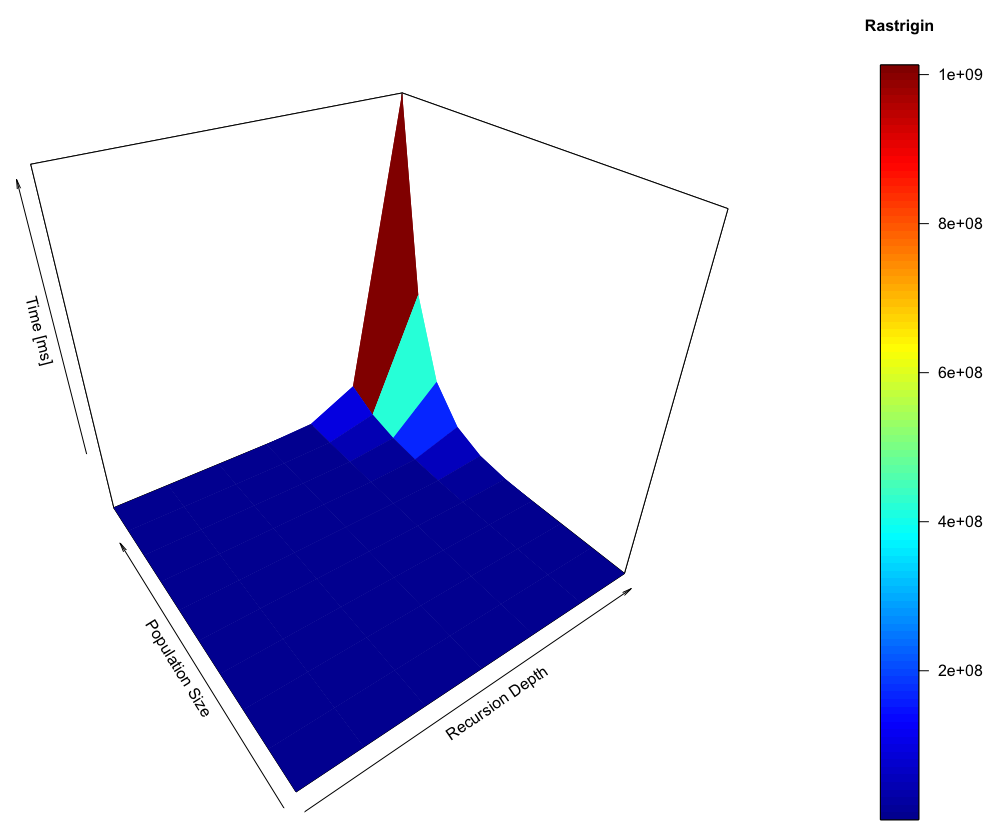
\includegraphics[width=1.0\textwidth,height=0.45\textheight]{images/fig04}
\caption{Rastrigin optimization time in milliseconds}
\label{fig:11}
\end{figure}
%\FloatBarrier

\begin{figure}[b]
\sidecaption
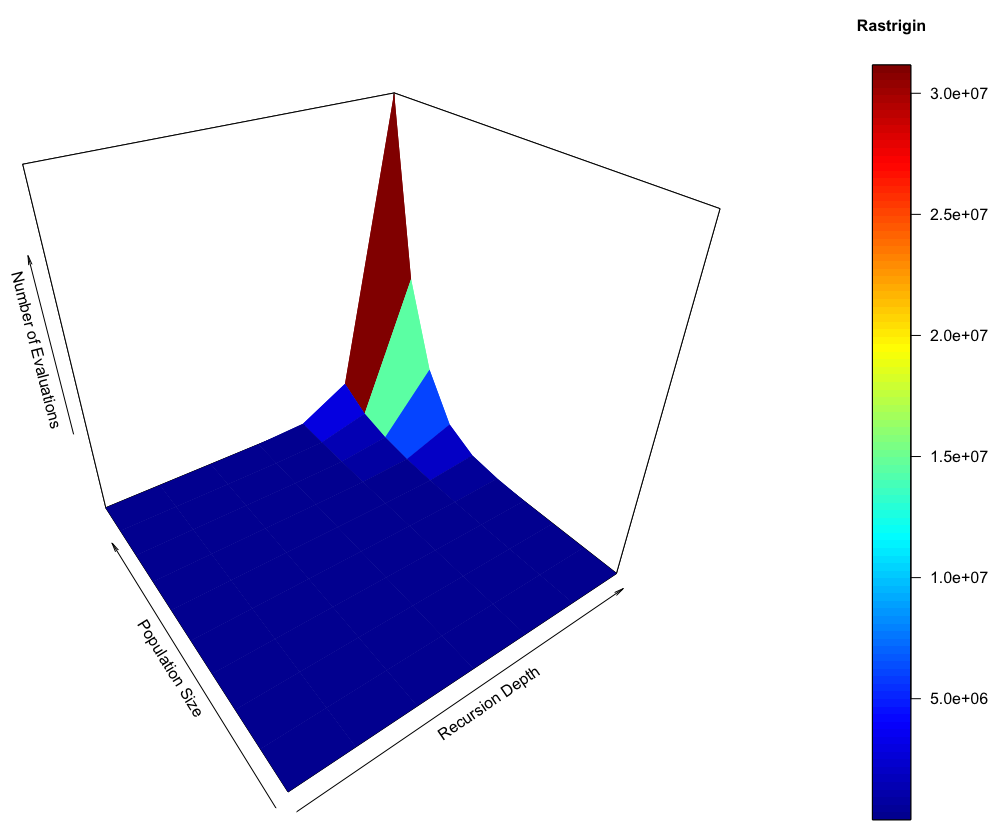
\includegraphics[width=1.0\textwidth,height=0.45\textheight]{images/fig05}
\caption{Rastrigin number of evaluated individuals}
\label{fig:12}
\end{figure}
%\FloatBarrier

\begin{figure}[b]
\sidecaption
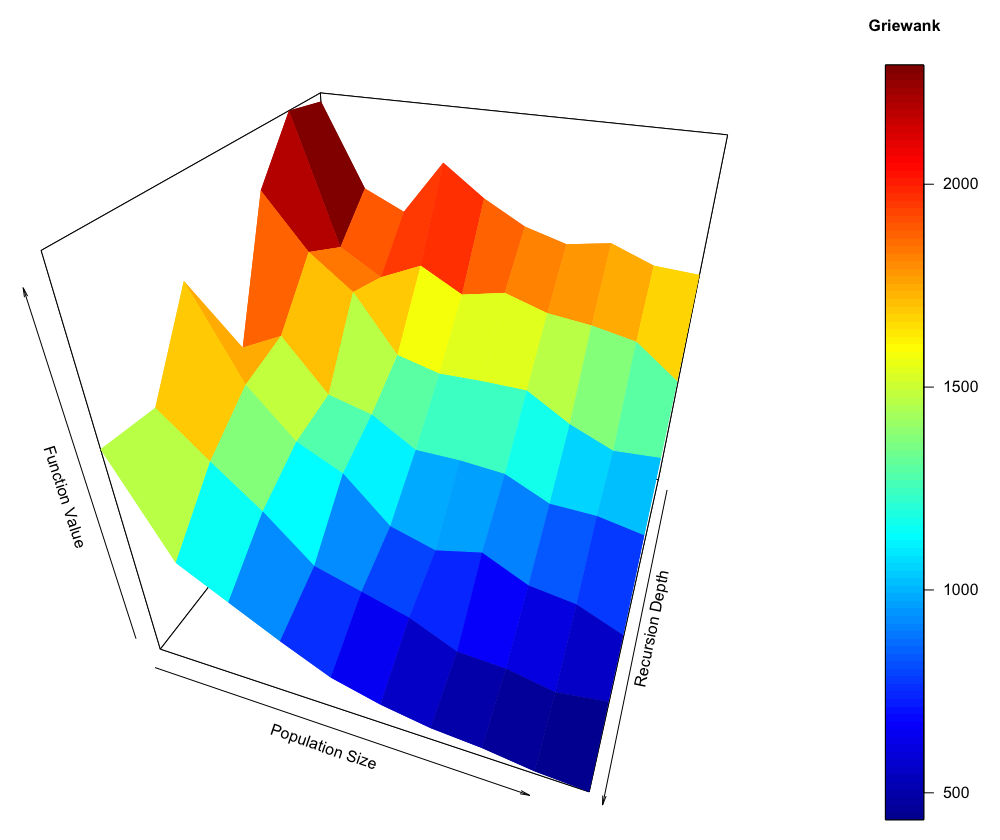
\includegraphics[width=1.0\textwidth,height=0.45\textheight]{images/fig06}
\caption{Griewank sub-optimal solutions found}
\label{fig:13}
\end{figure}
%\FloatBarrier

\begin{figure}[b]
\sidecaption
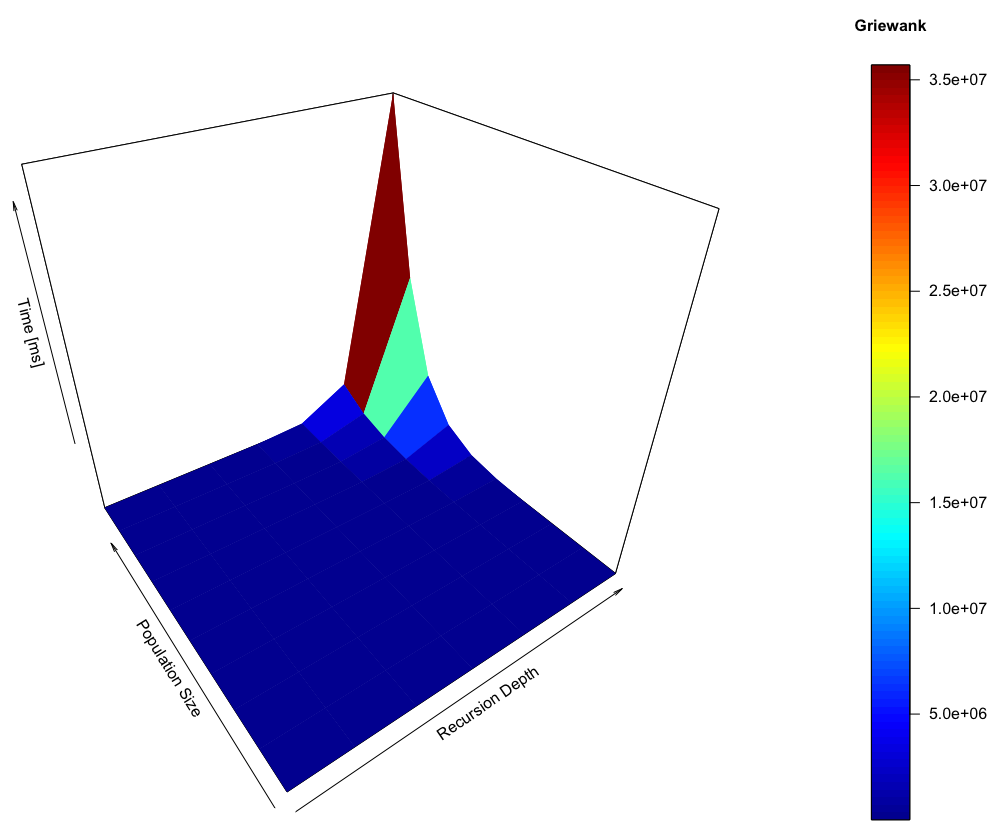
\includegraphics[width=1.0\textwidth,height=0.45\textheight]{images/fig07}
\caption{Griewank optimization time in milliseconds}
\label{fig:14}
\end{figure}
%\FloatBarrier

\begin{figure}[b]
\sidecaption
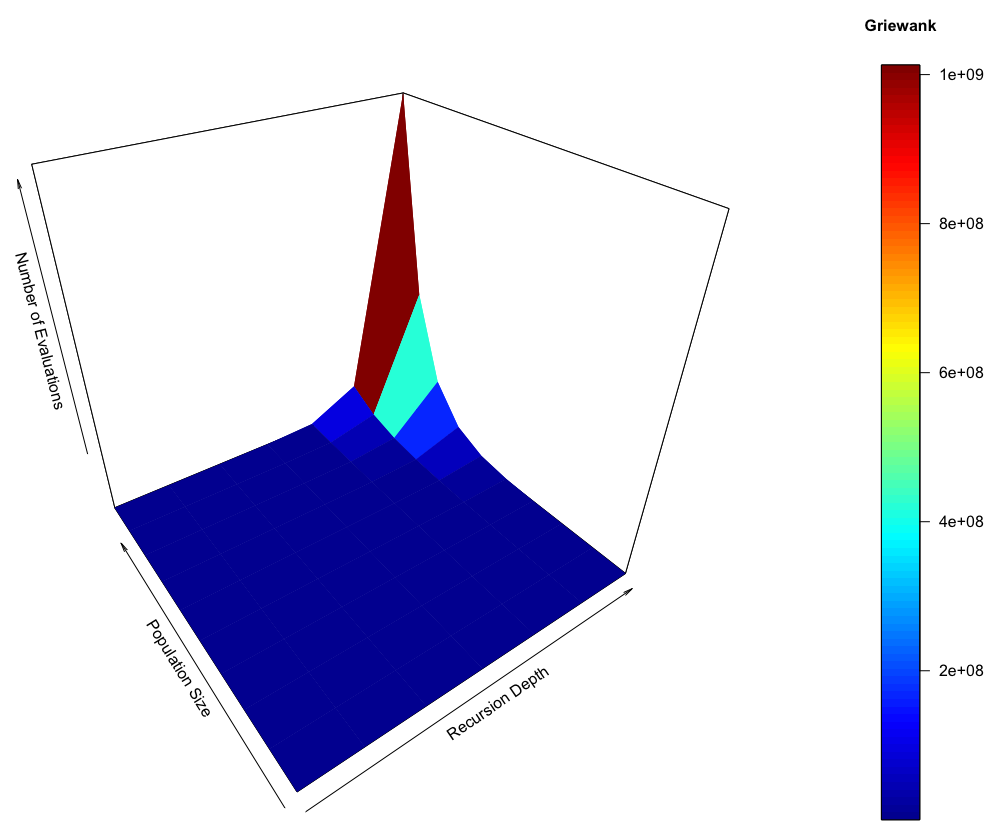
\includegraphics[width=1.0\textwidth,height=0.45\textheight]{images/fig08}
\caption{Griewank number of evaluated individuals}
\label{fig:15}
\end{figure}
%\FloatBarrier

Fig. \ref{fig:10} shows the sub-optimal values achieved for the Rastrigin function, and in a similar manner Fig. \ref{fig:13} shows the sub-optimal values achieved for the Griewank function. Fig. \ref{fig:11} and \ref{fig:14} graphically depict the computational time used to search for optimums for both functions. In terms of the number of individuals evaluated, the experiments for the two functions do not differ, as can be seen from Fig. \ref{fig:12} and \ref{fig:15}.

Despite the complexity of the two test functions, the graphs clearly show that the more individuals are generated and evaluated, the greater the approximation to the global optimum is.

\section{Conclusions}
\label{sec:4}

This study proposes a genetic algorithm selection operation that is based on recursive descent and complete depletion for each level of recursion. The experiments conducted clearly show that this type of selection operation gives promising results for the search in sub-optimal solutions for problems characterized by many local optima. Due to high computation time, this type of selection operation is best used in hybrid algorithms, where the initial population is not randomly generated but generated precisely by recursive selection and complete recombination in the individual levels of hierarchical invocation.

As a guide for future research, it would be appropriate to look for alternatives to complete depletion, which would reduce computational time.

\begin{acknowledgement}
This work was supported by a private funding of Velbazhd Software LLC. 
\end{acknowledgement}

\biblstarthook{}

\begin{thebibliography}{99.}
\end{thebibliography}

\end{document}
